\chapter{Análisis}
En este capítulo se analizan los requisitos del sistema que se va a desarrollar, es decir, las condiciones y capacidades que Liber debe satisfacer para cubrir las necesidades de las bibliotecas a las que se orienta. Se abordan tanto los requisitos funcionales (las operaciones que el sistema debe ser capaz de realizar) como los requisitos no funcionales, entre los que se incluyen los relativos a la interfaz de usuario, información gestionada, seguridad y restricciones de despliegue. Al haberse desarrollado iterativamente, se incluyen tanto los requisitos del prototipo inicial como los añadidos posteriormente. Asimismo, se especifican las condiciones de contorno del proyecto: la aplicación se concibe como un sistema multiplataforma accesible desde cualquier navegador \textit{web}, concebido en español y sin restricciones de uso, dado que se libera bajo licencia GPL y se orienta a una gran diversidad de instituciones. Para una descripción ordenada y comprensible de los requisitos, se emplean los denominados casos de uso, que permiten estructurar el análisis en torno a la identificación de los actores que interactúan con el sistema y las tareas que cada uno de ellos desempeña. Así se facilita la trazabilidad entre las necesidades detectadas, los objetivos definidos en el capítulo anterior y los criterios de aceptación que se emplearán en la fase de pruebas.
\section{Actores del sistema}
Los casos de uso que se describirán en este capítulo están íntegramente determinados por los usuarios, quienes los desempeñan. Los casos de uso describen las interacciones entre los usuarios y el sistema, por lo que es primordial describir qué usuarios intervienen así como sus características.
Se debe tener en cuenta que hay ciertos usuarios que cuyos casos de usuario son un subconjunto de los asignados a otros usuarios con más permisos de acción dentro del sistema diseñado.
Aquí se muestran los actores que intervienen en el sistema:
\begin{itemize}
	\item \textbf{Socio invitado:} Usuario no autenticado que puede acceder a acciones sencilla de visionado de datos, tales como consultar el catálogo, ver ejemplares o autores. Esto permite ver el fondo de la biblioteca sin tener que registrarse, especialmente útil para hacer una consulta sin tener que darse de alta. Otra funcionalidad destacable para este perfil es registrarse como socio, lo que da pie al siguiente tipo de usuario
	\item \textbf{Socio:} Usuario autenticado, es representado por una instancia en la base de datos del sistema. Puede realizar funciones más allá de ver el catálogo, siendo la más característica iniciar sesión y recuperar la contraseña, y otras como pedir prestado un ejemplar o solicitar su reserva.
	\item \textbf{Bibliotecario:} Los bibliotecarios pueden hacer todo lo que los socios, además de funciones administrativas como registrar ejemplares o gestionar los préstamos de los usuarios, o ver su información.
	\item \textbf{Administrador:} Es un tipo de usuario que puede modificar toda la base de datos del sistema, independientemente de la tabla que maneje. Este usuario tiene más permisos que cualquier otro, por lo que puede acceder a todos los casos de uso, excepto al registro por motivos obvios. Al ser un rol con tantos permisos, su registro no puede hacerse a través de la aplicación.
\end{itemize}
Al estar ante un conjunto de casos de uso similares que en ciertos momentos son puestos en práctica por diferentes tipos de usuario, lo más lógico ha sido recurrir a la herencia entre ciertos usuarios para simplificar la estructura conceptual de estos casos de uso. Los diferentes tipos de usuario que interactúan con la aplicación son los siguientes:
\begin{figure}[htb]
	\centering
		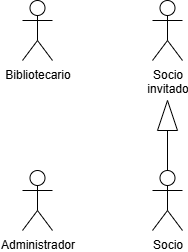
\includegraphics[scale=0.7]{imagenes/actores.png}
	\caption{Actores del sistema}
\end{figure}
En el diagrama se evidencia que el actor socio tendrá acceso a los mismos casos de uso que el socio invitado, pero sumando otros casos de uso propios.
\section{Requisitos de usuario}
Los requisitos de usuario reflejan las expectativas que tiene cada tipo de usuario a la hora de usar la aplicación; cómo espera que la misma se comporte cuando interactúa con ella, qué quiere encontrar... Estas necesidades de interacción y comportamiento del usuario a la aplicación se puede traducir en casos de uso.
\section{Casos de uso}
Ya definidos los actores que van a interactuar con el sistema, se procede a introducir los casos de uso.
Como introduce Francisco González \parencite{gonzalez2024casosuso} en los apuntes de su asignatura, un caso de uso representa una tarea o unidad coherente de funcionalidad que debe proporcionar el sistema a los actores, pudiendo participar varios actores diferentes en el mismo caso de uso. En este contexto, constituye una forma sencilla e intuitiva de documentar las funcionalidades que constituyen este sistema.
Se enumeran aquí los casos de uso desarrollados:
\begin{itemize}
	\item \textbf{CU01 -- Registrarse}
	\begin{itemize}
		\item \textbf{Actor:} Socio invitado.
		\item \textbf{Descripción:} Permite a un nuevo socio registrarse mediante un formulario, proporcionando datos como nombre, correo electrónico y contraseña. Si los datos son válidos, se crea el usuario y se inicia sesión automáticamente.
	\end{itemize}
	
	\item \textbf{CU02 -- Inicio de sesión}
	\begin{itemize}
		\item \textbf{Actor:} Bibliotecario, Administrador, Socio.
		\item \textbf{Descripción:} Permite a un socio acceder al sistema introduciendo sus credenciales. El sistema valida los datos y, en caso correcto, concede acceso según su rol (socio, bibliotecario o administrador).
	\end{itemize}
		
	\item \textbf{CU03 -- Recuperar contraseña}
	\begin{itemize}
		\item \textbf{Actor: Bibliotecario, Administrador, Socio.} 
		\item \textbf{Descripción: Mecanismo mediante el cual el usuario puede solicitar un enlace de recuperación de contraseña en caso de pérdida de la misma. Se envía un correo con este enlace, por lo que el usuario debe escribir el correo asociado a su cuenta para recibirlo.} 
	\end{itemize}
		
	\item \textbf{CU04 -- Consultar catálogo}
	\begin{itemize}
		\item \textbf{Actor:} Todos.
		\item \textbf{Descripción:} Permite buscar y visualizar los recursos disponibles en la biblioteca (obras y ejemplares). A partir de este caso de uso se pueden extender acciones como ver autores o ver ejemplares.
	\end{itemize}
	
	\item \textbf{CU05 -- Ver autores}
	\begin{itemize}
		\item \textbf{Actor:} Todos.
		\item \textbf{Descripción:} Permite consultar la información detallada de los autores asociados a las obras del catálogo. Extiende de la consulta de catálogo.
	\end{itemize}
	
	\item \textbf{CU06 -- Ver autor}
	\begin{itemize}
		\item \textbf{Actor:} Todos.
		\item \textbf{Descripción:} Permite consultar la información detallada de un autor determinado, como las obras pertenecientes a su autoría.
	\end{itemize}
	
	\item \textbf{CU07 -- Ver ejemplares}
	\begin{itemize}
		\item \textbf{Actor:} Todos.
		\item \textbf{Descripción:} Permite visualizar los ejemplares físicos concretos asociados a una obra, mostrando su estado y disponibilidad. Extiende de la consulta de catálogo.
	\end{itemize}
	
	\item \textbf{CU08 -- Consultar disponibilidad}
	\begin{itemize}
		\item \textbf{Actor:} Todos.
		\item \textbf{Descripción:} Permite comprobar si un ejemplar concreto se encuentra disponible para su préstamo o reserva en el momento de la consulta.
	\end{itemize}
	
	\item \textbf{CU09 -- Ver mi información personal}
	\begin{itemize}
		\item \textbf{Actor:} Administrador, Bibliotecario, Socio.
		\item \textbf{Descripción:} Permite al usuario acceder a los datos personales registrados en su perfil. A partir de esta vista se puede extender la modificación de los datos o la baja en el sistema, dependiendo del tipo de usuario.
	\end{itemize}
	
	\item \textbf{CU10 -- Modificar información personal}
	\begin{itemize}
		\item \textbf{Actor:} Administrador, Bibliotecario, Socio.
		\item \textbf{Descripción:} Permite al usuario actualizar sus datos personales (como dirección, correo o contraseña). Extiende de la visualización de la información personal. Algunos campos del formulario en el que consiste la vista del caso de uso cambia dependiendo del tipo de usuario.
	\end{itemize}
	
	\item \textbf{CU11 -- Darse de baja}
	\begin{itemize}
		\item \textbf{Actor:} Socio.
		\item \textbf{Descripción:} Permite al socio solicitar la eliminación o desactivación de su cuenta en el sistema. Extiende de la visualización de la información personal.
	\end{itemize}
	
	\item \textbf{CU12 -- Ver socios}
	\begin{itemize}
		\item \textbf{Actor:} Bibliotecario, Administrador.
		\item \textbf{Descripción:} Permite al usuario acceder al listado de todos los socios registrados en la biblioteca. A partir de esta vista se pueden extender las acciones de ver, modificar o eliminar un socio concreto.
	\end{itemize}
	
	\item \textbf{CU13 -- Ver socio}
	\begin{itemize}
		\item \textbf{Actor:} Bibliotecario, Administrador.
		\item \textbf{Descripción:} Permite visualizar la ficha detallada de un socio. Extiende del listado de socios.
	\end{itemize}
	
	\item \textbf{CU14 -- Modificar socio}
	\begin{itemize}
		\item \textbf{Actor:} Bibliotecario, Administrador.
		\item \textbf{Descripción:} Permite editar los datos de un socio registrado. Extiende de la visualización de un socio.
	\end{itemize}
	
	\item \textbf{CU15 -- Eliminar socio}
	\begin{itemize}
		\item \textbf{Actor:} Bibliotecario, Administrador.
		\item \textbf{Descripción:} Permite dar de baja a un socio del sistema. Extiende de la visualización de un socio.
	\end{itemize}
		
	\item \textbf{CU16 -- Modificación, visionado y borrado sobre bibliotecarios y administradores}
	\begin{itemize}
		\item \textbf{Actor:} Administrador.
		\item \textbf{Descripción:} Permite ver, modificar y eliminar bibliotecarios y administradores al administrador, extiende de ver usuarios.
	\end{itemize}
	
	\item \textbf{CU17-- Nuevo socio}
	\begin{itemize}
		\item \textbf{Actor:} Bibliotecario, Administrador.
		\item \textbf{Descripción:} Permite registrar manualmente a un nuevo socio en el sistema, recopilando sus datos personales.
	\end{itemize}
	
	\item \textbf{CU18 -- Gestionar catálogo / Registrar ejemplar}
	\begin{itemize}
		\item \textbf{Actor:} Bibliotecario, Administrador.
		\item \textbf{Descripción:} Permite dar de alta un nuevo ejemplar físico en el sistema. A partir de esta acción se pueden extender el registro de nuevos autores, editoriales o productoras.
	\end{itemize}
	
	\item \textbf{CU19 -- Registrar autor/editorial/productora}
	\begin{itemize}
		\item \textbf{Actor:} Bibliotecario, Administrador.
		\item \textbf{Descripción:} Permite añadir los datos de las entidades relacionadas con las obras (autores, editoriales o productoras) para poder vincularlas a los ejemplares. Extiende del registro de ejemplares.
	\end{itemize}
	
	\item \textbf{CU20 -- Duplicar ejemplar}
	\begin{itemize}
		\item \textbf{Actor:} Bibliotecario, Administrador.
		\item \textbf{Descripción:} Permite crear un nuevo registro de ejemplar tomando como base los datos de uno ya existente (por ejemplo, para añadir copias del mismo libro).
	\end{itemize}
	
	\item \textbf{CU21 -- Dar de alta bibliotecario}
	\begin{itemize}
		\item \textbf{Actor:} Administrador.
		\item \textbf{Descripción:} Permite al administrador registrar a un nuevo usuario con rol de bibliotecario, garantizando que solo personal autorizado tenga acceso a las funciones de gestión.
	\end{itemize}
	
	\item \textbf{CU22 -- CRUD sobre BBDD a través del panel de admin}
	\begin{itemize}
		\item \textbf{Actor:} Administrador.
		\item \textbf{Descripción:} Proporciona al administrador acceso total al panel de administración de Django para realizar operaciones de creación, lectura, actualización y borrado sobre cualquier registro del sistema.
	\end{itemize}
		
	\item \textbf{CU23 -- CRUD sobre todo tipo de usuarios}
	\begin{itemize}
		\item \textbf{Actor:} Administrador.
		\item \textbf{Descripción:} Permite al administrador gestionar de forma completa cualquier perfil de usuario del sistema (socios, bibliotecarios u otros administradores). Extiende del CRUD general sobre la base de datos.
	\end{itemize}
	
	\item \textbf{CU24 -- Prestar ejemplar a socio}
	\begin{itemize}
		\item \textbf{Actor:} Bibliotecario, Administrador.
		\item \textbf{Descripción:} Permite registrar el préstamo de un ejemplar a un socio. Incluye obligatoriamente la verificación de la disponibilidad del ejemplar.
	\end{itemize}
	
	\item \textbf{CU25 -- Devolver ejemplar}
	\begin{itemize}
		\item \textbf{Actor:} Bibliotecario, Administrador.
		\item \textbf{Descripción:} Permite registrar la devolución de un ejemplar prestado, actualizando su estado a disponible. Puede extenderse si el socio devuelve el ejemplar con retraso (aplicando penalización).
	\end{itemize}
	
	\item \textbf{CU26 -- Consultar mis préstamos}
	\begin{itemize}
		\item \textbf{Actor:} Socio.
		\item \textbf{Descripción:} Permite al socio consultar el estado de los préstamos que tiene activos. A partir de aquí puede extenderse la solicitud de prórroga.
	\end{itemize}
	
	\item \textbf{CU27 -- Consultar préstamos de socio}
	\begin{itemize}
		\item \textbf{Actor:} Bibliotecario, Administrador.
		\item \textbf{Descripción:} Permite al usuario consultar el historial y estado de los préstamos de un socio concreto.
	\end{itemize}
	
	
	\item \textbf{CU28 -- Solicitar prórroga}
	\begin{itemize}
		\item \textbf{Actor:} Administrador, Bibliotecario, Socio.
		\item \textbf{Descripción:} Permite al socio extender el plazo de devolución de un préstamo activo, siempre que se cumplan las condiciones establecidas. Extiende de la consulta de préstamos. El socio también puede solicitar esta acción a un bibliotecario, que tiene acceso a todos los préstamos de los socios.
	\end{itemize}

	\item \textbf{CU29 -- Ver préstamo}
	\begin{itemize}
		\item \textbf{Actor:} Bibliotecario.
		\item \textbf{Descripción:} Permite visualizar el detalle de un préstamo y prorrogar su fecha de devolución a petición del socio. Extiende de la consulta de préstamos de socio.
	\end{itemize}
	
\end{itemize}

Para dar una representación sencilla y visual de qué usuario desempeña cada caso de uso, se ha elaborado la tabla \ref{tab:relacion_cu_actores}, que lo muestra expresamente.
Adicionalmente, más adelante se puede encontrar un diagrama que ilustra la relación entre actores y casos de uso de una forma más visual. El lenguaje visual utilizado es \textit{UML (Unified Modeling Language)}, un estándar en la industria para modelar sistemas \textit{software} de todo tipo. Específicamente, se trata de un diagrama \textit{UML} de casos de uso, por lo que tiene sus propias reglas y elementos.
Este tipo de diagrama tiene como objetivo mostrar una vista genérica del funcionamiento del sistema elaborado a través de cómo se relacionan los actores con el mismo. Se pueden distinguir los siguientes elementos en el diagrama:

\begin{itemize}
	\item \textbf{Actores:} Representan los roles que adoptan las entidades externas (ya sean personas, sistemas hardware o software) que interactúan con la aplicación. Se representan gráficamente mediante monigotes y se sitúan fuera del límite del sistema. En el contexto de Liber, los actores principales son el Socio, el Bibliotecario y el Administrador (además del Socio invitado).
	
	\item \textbf{Sistema (o Límite del sistema):} Se representa mediante un rectángulo que engloba todos los casos de uso. Define las fronteras de la aplicación, es decir, qué funcionalidades pertenecen al sistema que se está modelando y cuáles son responsabilidad del entorno externo.
	
	\item \textbf{Casos de uso:} Son las funcionalidades o unidades de comportamiento que el sistema ofrece a sus actores. Se representan mediante elipses y su nombre suele ser una frase verbal (por ejemplo, ``Registrarse'', o ``Prestar ejemplar'').
	
	\item \textbf{Relaciones:} Son las líneas que conectan los elementos anteriores y definen cómo interactúan entre sí. Se distinguen tres tipos principales en este diagrama:
	\begin{itemize}
		\item \textbf{Asociación (Actor - Caso de uso):} Una línea continua que une un actor con un caso de uso, indicando que dicho actor interactúa con esa funcionalidad del sistema.
		\item \textbf{Inclusión (\texttt{<<include>>}):} Una flecha discontinua que apunta desde un caso de uso base hacia un caso de uso incluido. Se utiliza cuando un caso de uso contiene obligatoriamente el comportamiento de otro (por ejemplo, ``Prestar ejemplar'' incluye obligatoriamente ``Comprobar disponibilidad''). Evita duplicar comportamientos comunes.
		\item \textbf{Extensión (\texttt{<<extend>>}):} Una flecha discontinua que apunta desde un caso de uso de extensión hacia el caso de uso base. Se utiliza para indicar un comportamiento opcional o alternativo que solo ocurre bajo ciertas condiciones (por ejemplo, ``Renovar préstamo'' extiende de ``Consultar mis préstamos'', ya que no siempre se renueva).
	\end{itemize}
\end{itemize}
\begin{table}[H]
	\centering
	\caption{Relación de casos de uso y roles de usuario.}
	\label{tab:relacion_cu_actores}
	\small
	\begin{tabularx}{\textwidth}{X c c c c}
		\toprule
		\textbf{Caso de Uso} & \textbf{Invitado} & \textbf{Socio} & \textbf{Bibliotecario} & \textbf{Administrador} \\
		\midrule
		CU01 -- Registrarse & \checkmark & & & \\
		\addlinespace
		CU02 -- Inicio de sesión & & \checkmark & \checkmark & \checkmark \\
		\addlinespace
		CU03 -- Recuperar contraseña & & \checkmark & \checkmark & \checkmark \\
		\addlinespace
		CU04 -- Consultar catálogo & \checkmark & \checkmark & \checkmark & \checkmark \\
		\addlinespace
		CU05 -- Ver autores & \checkmark & \checkmark & \checkmark & \checkmark \\
		\addlinespace
		CU06 -- Ver autor & \checkmark & \checkmark & \checkmark & \checkmark \\
		\addlinespace
		CU07 -- Ver ejemplares & \checkmark & \checkmark & \checkmark & \checkmark \\
		\addlinespace
		CU08 -- Consultar disponibilidad & \checkmark & \checkmark & \checkmark & \checkmark \\
		\addlinespace
		CU09 -- Ver mi información personal & & \checkmark & \checkmark & \checkmark \\
		\addlinespace
		CU10 -- Modificar información personal & & \checkmark & \checkmark & \checkmark \\
		\addlinespace
		CU11 -- Darse de baja & & \checkmark & & \\
		\addlinespace
		CU12 -- Ver socios & & & \checkmark & \checkmark \\
		\addlinespace
		CU13 -- Ver socio & & & \checkmark & \checkmark \\
		\addlinespace
		CU14 -- Modificar socio & & & \checkmark & \checkmark \\
		\addlinespace
		CU15 -- Eliminar socio & & & \checkmark & \checkmark \\
		\addlinespace
		CU16 -- Modificación, visionado y borrado sobre bibliotecarios y administradores & & & & \checkmark \\
		\addlinespace
		CU17 -- Nuevo socio & & & \checkmark & \checkmark \\
		\addlinespace
		CU18 -- Gestionar catálogo / Registrar ejemplar & & & \checkmark & \checkmark \\
		\addlinespace
		CU19 -- Registrar autor/editorial/productora & & & \checkmark & \checkmark \\
		\addlinespace
		CU20 -- Duplicar ejemplar & & & \checkmark & \checkmark \\
		\addlinespace
		CU21 -- Dar de alta bibliotecario & & & & \checkmark \\
		\addlinespace
		CU22 -- CRUD sobre BBDD a través del panel de admin & & & & \checkmark \\
		\addlinespace
		CU23 -- CRUD sobre todo tipo de usuarios & & & & \checkmark \\
		\addlinespace
		CU24 -- Prestar ejemplar a socio & & & \checkmark & \checkmark \\
		\addlinespace
		CU25 -- Devolver ejemplar & & & \checkmark & \checkmark \\
		\addlinespace
		CU26 -- Consultar mis préstamos & & \checkmark & & \\
		\addlinespace
		CU27 -- Consultar préstamos de socio & & & \checkmark & \checkmark \\
		\addlinespace
		CU28 -- Solicitar prórroga & & \checkmark & \checkmark & \checkmark \\
		\addlinespace
		CU29 -- Ver préstamo & & & \checkmark & \\
		\bottomrule
	\end{tabularx}
\end{table}

\begin{figure}[H]
	\centering
	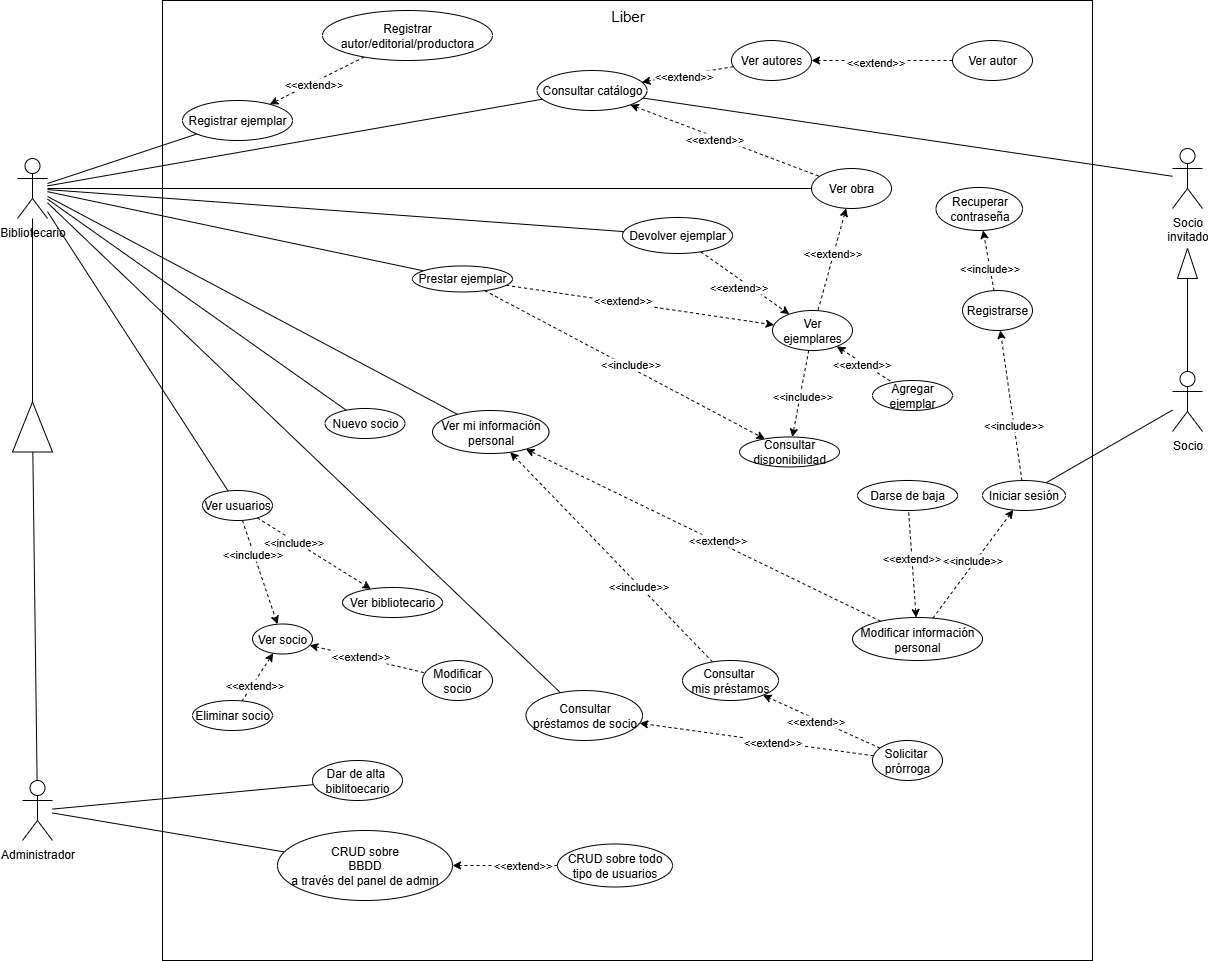
\includegraphics[width=\textwidth]{imagenes/casos_uso.png}
	\caption{Diagrama de casos de uso del sistema Liber.}
	\label{fig:diagrama_casos_uso}
\end{figure}

\section{Historias de usuario}

\section{Objetivos del trabajo}

Al estar tratando con proyecto de estas dimensiones, se hace necesaria una planificación estructurada a seguir para marcar tanto los plazos a cumplir como las restricciones y casos de uso específicos a tener en cuenta.	

\begin{table}[H]
	\centering
	\caption{Criterios de aceptación para el objetivo general OBJ-01.}
	\label{tab:criterios_aceptacion_normal01}
	\begin{tabularx}{\textwidth}{l X}
		\toprule
		\textbf{ID C.A.} & 
		\begin{minipage}[t]{\linewidth}
			\textbf{ID Objetivo asociado: OBJ-01} \\[2pt]
			\rule{\linewidth}{0.4pt} \\[2pt]
			\textbf{Descripción Criterio de Aceptación}
		\end{minipage} \\
		\midrule
		\textbf{CA-01} & El sistema debe permitir el alta, modificación, consulta y baja (CRUD) de Obras intelectuales, almacenando de forma obligatoria su título y signatura. \\
		\addlinespace
		\textbf{CA-02} & El sistema debe permitir la creación de Ejemplares físicos asociados obligatoriamente a una Obra preexistente, permitiendo marcar su estado de disponibilidad. \\
		\addlinespace
		\textbf{CA-03} & La aplicación debe gestionar correctamente la especialización de los ejemplares (Libros, Revistas, Periódicos y Grabaciones) cargando dinámicamente sus atributos específicos en la base de datos. \\
		\addlinespace
		\textbf{CA-04} & El catálogo debe soportar la relación de coautoría (relación N:M), permitiendo que una misma Obra sea vinculada a uno o varios Autores simultáneamente. \\
		\addlinespace
		\textbf{CA-05} & La interfaz del catálogo debe permitir a los usuarios realizar búsquedas funcionales y filtrados de los ejemplares empleando la interactividad en el frontal propia de Django. \\
		\addlinespace
		\textbf{CA-06} & El sistema debe validar a nivel de formulario y de base de datos que los identificadores estándar del catálogo (como el ISBN o el EAN) mantengan su propiedad de unicidad para garantizar la integridad de la información. \\
		\bottomrule
	\end{tabularx}
\end{table}

\begin{table}[H]
	\centering
	\caption{Criterios de aceptación para el objetivo general OBJ-02.}
	\label{tab:criterios_aceptacion_normal02}
	\begin{tabularx}{\textwidth}{l X}
		\toprule
		\textbf{ID C.A.} & 
		\begin{minipage}[t]{\linewidth}
			\textbf{ID Objetivo asociado: OBJ-02} \\[2pt]
			\rule{\linewidth}{0.4pt} \\[2pt]
			\textbf{Descripción Criterio de Aceptación}
		\end{minipage} \\
		\midrule
		\textbf{CA-01} & El sistema debe implementar un único modelo de base de datos centralizado para la entidad usuario que almacene obligatoriamente el nombre, los apellidos, una contraseña cifrada y un correo electrónico único que actúe como credencial de inicio de sesión. \\
		\addlinespace
		\textbf{CA-02} & El sistema debe permitir el acceso específico de los socios, validando que posean un número identificativo único y bloqueando automáticamente sus privilegios de reserva o préstamo en caso de que consten como penalizados en la base de datos. \\
		\addlinespace
		\textbf{CA-03} & La interfaz y los formularios para los bibliotecarios deben permitir, de manera exclusiva, la gestión ordinaria del catálogo y el registro de las transacciones de préstamo, validando su identidad mediante unas credenciales de acceso. \\
		\addlinespace
		\textbf{CA-04} & El rol de ADMINISTRADOR debe disponer de acceso total e irrestricto a través del panel de control de Django para realizar operaciones CRUD completas sobre cualquier tabla o registro de la infraestructura. \\
		\addlinespace
		\textbf{CA-05} & El backend debe denegar el acceso a rutas protegidas mediante un sistema de control de permisos (middleware), redirigiendo al usuario a la pantalla de inicio de sesión si intenta forzar manualmente URLs no autorizadas para su rol. \\
		\addlinespace
		\textbf{CA-06} & El sistema debe garantizar que las contraseñas de los usuarios nunca se almacenen en texto plano dentro de la base de datos PostgreSQL, delegando en el framework el cifrado automático mediante algoritmos de hash seguros. \\
		\bottomrule
	\end{tabularx}	
\end{table}

\begin{table}[H]
	\centering
	\caption{Criterios de aceptación para el objetivo general OBJ-3.}
	\label{tab:criterios_aceptacion_normal03}
	\begin{tabularx}{\textwidth}{l X}
		\toprule
		\textbf{ID C.A.} & 
		\begin{minipage}[t]{\linewidth}
			\textbf{ID Objetivo asociado: OBJ-3} \\[2pt]
			\rule{\linewidth}{0.4pt} \\[2pt]
			\textbf{Descripción Criterio de Aceptación}
		\end{minipage} \\
		\midrule
		\textbf{CA-01} & El sistema debe registrar automáticamente la transacción en la tabla de préstamos en el momento en que un bibliotecario la gestione, asignando la fecha actual a la fecha de inicio del préstamo. \\
		\addlinespace
		\textbf{CA-02} & La aplicación debe calcular de forma automática la fecha límite de devolución sumando el número de días estipulado por la política de la biblioteca a partir de la fecha de inicio de la transacción. \\
		\addlinespace
		\textbf{CA-03} & El sistema debe permitir la gestión de prórrogas antes de que termine el plazo del préstamo, verificando que el registro cuente con un número de prórrogas restantes mayor que cero, actualizando la fecha de la prórroga con la marca de tiempo actual y extendiendo la fecha de fin de manera proporcional. \\
		\addlinespace
		\textbf{CA-04} & Al solicitarse una prórroga válida, el backend debe descontar automáticamente en una unidad el contador de prórrogas disponibles para ese préstamo específico en la base de datos. \\
		\addlinespace
		\textbf{CA-05} & En el momento de la entrega física del recurso, el sistema debe registrar la fecha del día exacto en el campo de devolución. Si esta fecha es anterior o igual a la fecha límite, la transacción se considerará cerrada con éxito y el ejemplar volverá a estar disponible. \\
		\addlinespace
		\textbf{CA-06} & Si el sistema detecta que la devolución se realiza tarde (fecha de devolución posterior a la fecha límite), o que el plazo ha vencido sin haber devuelto el recurso, el backend debe activar de inmediato el estado de penalización del socio y registrar la fecha del bloqueo. \\
		\bottomrule
	\end{tabularx}	
\end{table}

\begin{table}[H]
	\centering
	\caption{Criterios de aceptación para el objetivo general OBJ-4.}
	\label{tab:criterios_aceptacion_normal04}
	\begin{tabularx}{\textwidth}{l X}
		\toprule
		\textbf{ID C.A.} & 
		\begin{minipage}[t]{\linewidth}
			\textbf{ID Objetivo asociado: OBJ-4} \\[2pt]
			\rule{\linewidth}{0.4pt} \\[2pt]
			\textbf{Descripción Criterio de Aceptación}
		\end{minipage} \\
		\midrule
		\textbf{CA-01} & El sistema debe disponer de un archivo Dockerfile en la parte backend que configure un entorno limpio basado en una imagen ligera de Python, instalando de forma automática todas las dependencias recolectadas en el archivo requirements.txt. \\
		\addlinespace
		\textbf{CA-02} & El entorno de la base de datos debe levantarse de forma aislada a través de un servicio independiente en el archivo docker-compose.yml, utilizando una imagen oficial y reciente de PostgreSQL. \\
		\addlinespace
		\textbf{CA-03} & El archivo docker-compose.yml debe orquestar la comunicación interna entre ambos contenedores (Django y PostgreSQL), garantizando que el contenedor web no intente arrancar hasta que el servicio de la base de datos esté completamente listo y operativo. \\
		\addlinespace
		\textbf{CA-04} & El contenedor de la base de datos debe implementar un volumen de Docker mapeado a la ruta de almacenamiento de PostgreSQL para asegurar la persistencia de los datos, impidiendo que el catálogo, los socios o los préstamos se borren al apagar o reiniciar los contenedores. \\
		\addlinespace
		\textbf{CA-05} & El sistema debe ser capaz de replicar exactamente el mismo comportamiento, rendimiento y configuración tanto al ser ejecutado en local (entorno de desarrollo) como al ser desplegado en plataformas en la nube sin necesidad de modificar el código fuente de la aplicación web. \\
		\bottomrule
	\end{tabularx}	
\end{table}

\begin{table}[H]
	\centering
	\caption{Criterios de aceptación para el objetivo general OBJ-5.}
	\label{tab:criterios_aceptacion_normal05}
	\begin{tabularx}{\textwidth}{l X}
		\toprule
		\textbf{ID C.A.} & 
		\begin{minipage}[t]{\linewidth}
			\textbf{ID Objetivo asociado: OBJ-5} \\[2pt]
			\rule{\linewidth}{0.4pt} \\[2pt]
			\textbf{Descripción Criterio de Aceptación}
		\end{minipage} \\
		\midrule
		\textbf{CA-01} & El proyecto debe incluir en su directorio raíz el archivo estandarizado LICENSE conteniendo el texto íntegro y oficial de la Licencia Pública General de GNU (GNU GPL v3), declarando formalmente el software como libre y abierto. \\
		\addlinespace
		\textbf{CA-02} & El código fuente de la aplicación Django debe subirse y estar disponible públicamente en una plataforma de control de versiones accesible (como GitHub o GitLab), permitiendo que cualquier usuario pueda clonar, bifurcar (fork) o descargar el repositorio sin restricciones. \\
		\addlinespace
		\textbf{CA-03} & Las vistas de Django, los modelos y las configuraciones de Docker deben contar con comentarios claros y documentación interna en las secciones complejas, simplificando la curva de aprendizaje para futuros miembros de la comunidad que deseen auditar o colaborar en el proyecto. \\
		\addlinespace
		\textbf{CA-04} & La configuración del sistema (como las claves secretas de Django o las credenciales de PostgreSQL) debe estar parametrizada mediante variables de entorno en un archivo .env.example, asegurando que cualquier usuario pueda desplegar su propia instancia de la biblioteca de forma local de manera inmediata y sin comprometer la seguridad. \\
		\bottomrule
	\end{tabularx}	
\end{table}

\begin{table}[H]
	\centering
	\caption{Criterios de aceptación para el objetivo general OBJ-6.}
	\label{tab:criterios_aceptacion_normal06}
	\begin{tabularx}{\textwidth}{l X}
		\toprule
		\textbf{ID C.A.} & 
		\begin{minipage}[t]{\linewidth}
			\textbf{ID Objetivo asociado: OBJ-6} \\[2pt]
			\rule{\linewidth}{0.4pt} \\[2pt]
			\textbf{Descripción Criterio de Aceptación}
		\end{minipage} \\
		\midrule
		\textbf{CA-01} & Demostrar la correcta aplicación de los fundamentos de ingeniería mediante el diseño e implementación del esquema lógico relacional en PostgreSQL, reflejando fielmente las restricciones de integridad y las relaciones de herencia. \\
		\addlinespace
		\textbf{CA-02} &  El desarrollo de la aplicación web debe evidenciar un desacoplamiento claro de responsabilidades siguiendo el patrón arquitectónico MVT (Modelo-Vista-Template) de Django, separando la lógica de acceso a datos de la lógica de presentación y de negocio. \\
		\textbf{CA-03} & La memoria del Trabajo de Fin de Grado debe documentar con rigor de ingeniería todas las fases del ciclo de vida del desarrollo de software, incluyendo el análisis de requisitos, el modelado formal (diagramas de casos de uso y de entidad-relación) y las pruebas de validación.  \\
		\addlinespace
		\bottomrule
	\end{tabularx}	
\end{table}

\section{Condiciones técnicas}

\section{Alcance y limitaciones}